\documentclass[varwidth]{standalone}
\usepackage{tikz}
\usepackage{pgfplots}
\begin{document}
    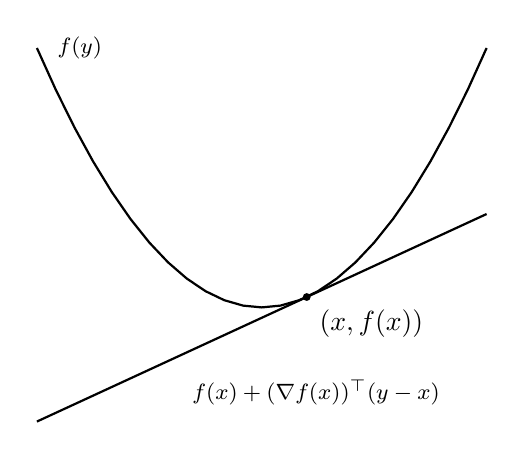
\begin{tikzpicture}
        \begin{axis}[axis lines = none]
            \addplot[thick] {0.5 * x^2} node[pos=0,label={0:{\footnotesize$f(y)$}}] {};
            \addplot[thick] {x - 0.5} node[pos=0.3,label={315:{\footnotesize$f(x) + (\nabla f(x))^\top (y - x)$}}] {};
            \node[label={315:{$(x, f(x))$}},fill, circle,inner sep=1pt] at (axis cs:1, 0.5) {};
        \end{axis}
    \end{tikzpicture}
\end{document}